\part{Introduction}
This work presents a study on the new system, OPEN-RMF, which is still under active development but has reached a mature enough state to be deployed in mobile robots at Elettra Sincrotrone Trieste.
\chapter{Background and motivation}
Elettra Sincontrone Trieste\footnote{\href{https://www.elettra.eu/}{https://www.elettra.eu/}} is a major research facility that primarily provides users access to two light sources: the synchrotron Elettra and the free electron laser FERMI.
In addition to operating these sources, the facility actively researches new technologies and techniques to enhance its capabilities and operations. Many recent advancements are based on robotics, which, especially after the COVID-19 pandemic and with the rapid rise of large language models (LLMs), have enabled new ways for users to interact with the infrastructure, including robot-assisted information retrieval and package delivery services.
Previously, the facility developed a global planner, D-Star (D-star based optimized trajectory planner)\cite{10.1007/978-3-031-45770-8_29}, within the ROS 1 framework to enable robot navigation across large-scale environments.  However, as ROS 1 has reached end-of-life, the codebase must now be migrated to ROS 2.
Additionally, the facility employs robots from multiple vendors, each specialized in different tasks and not designed to coordinate with one another.
An environment that has narrow passages and lifts can create significant coordination challenges during navigation.
To address this issue,  Open-RMF\footnote{\href{https://www.open-rmf.org/}{https://www.open-rmf.org/}} has been developed in recent years as a multiplatform system for controlling and managing heterogeneous fleets of robots.
\chapter{Research questions and objectives}
The objectives of this thesis are: to integrate a Rover Mini robot from the company RoverRobotics \footnote{\href{https://roverrobotics.com/}{https://roverrobotics.com/}}
into the ROS 2 Nav2 ecosystem,\\
\begin{figure}[h]
	\centering
	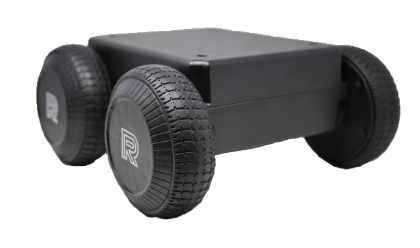
\includegraphics[width=0.4\linewidth]{img/RoverRoboticsMini.png}
	\captionof{figure}{RoverRobotics Rover Mini}
	\label{fig:RoverRobotics Rover Mini}
\end{figure}\\
to port the D-Star global planner from ROS 1 to ROS 2,
upgrade our Jobot rover from ROS 1 to ROS 2,\\
\begin{figure}[h]
	\centering
	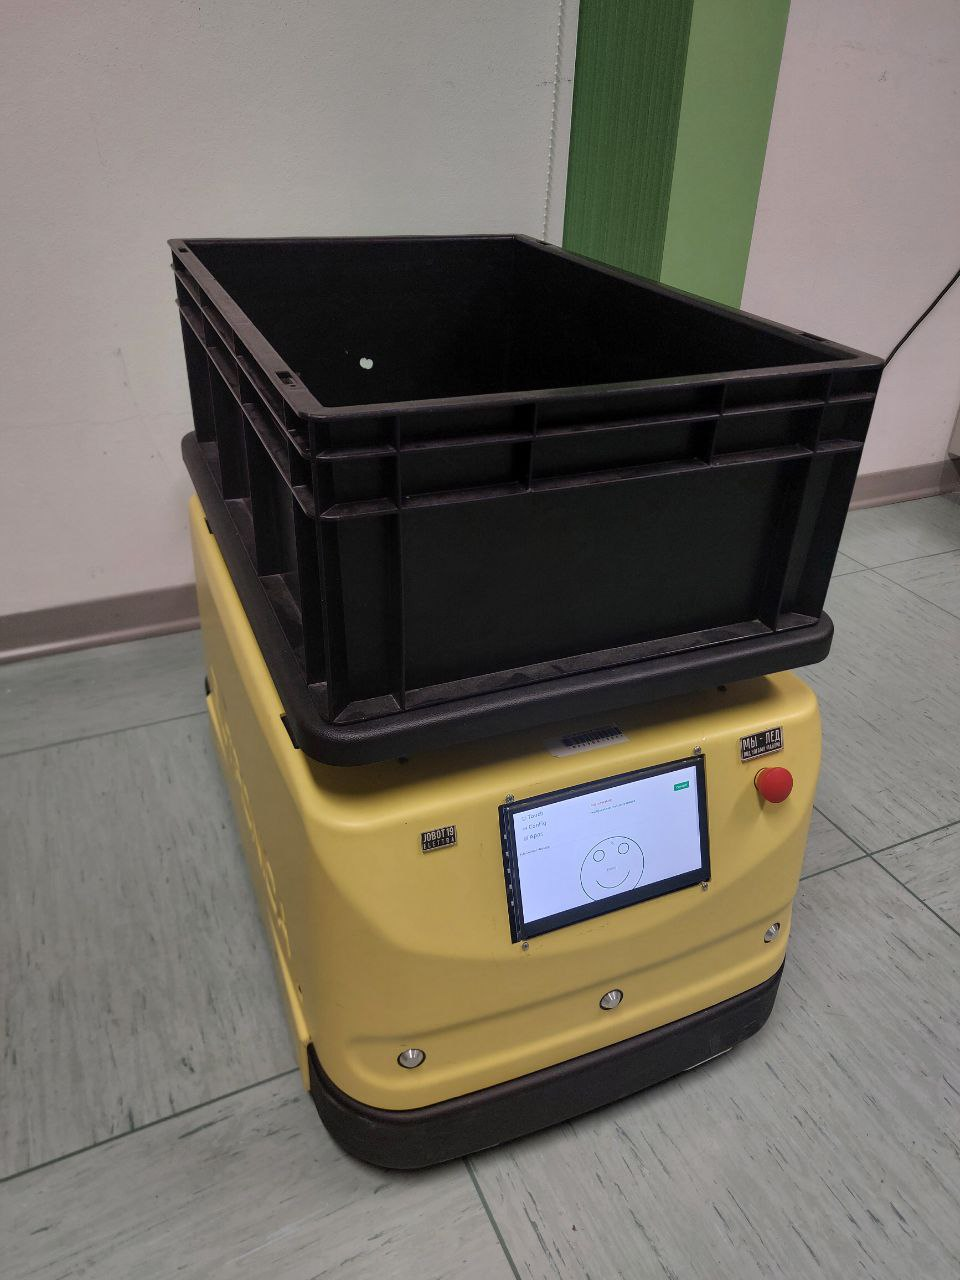
\includegraphics[width=0.3\linewidth]{img/jobot_robot.jpg}
	\captionof{figure}{Jobot Rover}
	\label{fig:Jobot Rover}
\end{figure}\\
incorporate the robot into the Open-RMF framework for centralized fleet management and evaluate the suitability of the Open-RMF ecosystem for deployment at the Elettra Sincrotrone Trieste.
\chapter{Scope and limitations}
The principal limitation is the current lack of access to lift control systems, which prevents direct integration and operation by the robot fleet. Additionally, there is no automated system for opening and closing doors. While Open-RMF offers a high degree of customizability, and human-in-the-loop interactions can be configured—such as triggering a light or sending a notification when a robot approaches a door—this method requires a human to manually open the door or operate the lift. However, such an approach is not ideal for achieving full autonomy.
